\lesson{Overview}
\begin{bulleted-list}
    \item Chemists coined the term \textbf{organic} to distinguish between compounds obtained from living
    organisms and those obtained from mineral sources
    \item Carbon is the central atom in the study of 
    organic chemistry
    \footnote{\textbf{Organic chemistry:} the study of compounds in which carbon is the principle 
    element.}
    because the carbon atom can form four bonds. They can bond to form chains, rings, spheres, sheets,
    and tubes of almost any size and can form combinations of single, double, and triple covalent bonds.
    \item \textbf{Terminal carbon} is where the chain of carbon ends
\end{bulleted-list}

\lesson{Functional Groups}
\begin{bulleted-list}
    \item Compounds fall into \textbf{organic families}
        \footnote{
            \textbf{Organic family:} a group of organic compounds with common structural features
            that impart characteristic physical properties and reactivity
        }
    \item The physical properties and reactivity of the compounds are related to these combinations,
        called \textbf{functional groups}
        \footnote{
            \textbf{Functional groups:} these groups determine whether the molecules are readily
            soluble in polar or non-polar solvents, whether they have high or low melting/boiling
            points, and whether they readily react with other molecules
        }
    \item Thus, if we can identify the functional group a organic compound belongs to, we can predict
        the properties of the molecule
\end{bulleted-list}
Each functional group can be composed of \textbf{3 different types of components}
\begin{enum}
    \item Carbon-carbon multiple bonds (single, double, and triple bonds). The diagram below
        shows the double bond between two carbons in ethene
        \begin{center}
            ethene, \ce{C2H4}

            \chemfig{H-C(-[:90]H)=C(-[:90]H)-H}
        \end{center}
    \item Single bonds between a carbon atom and a more electronegative atom. For instance, a
        \ce{C-O}, a \ce{C-N} bond, or a \ce{C-Cl} bond. The diagram below shows the bond between
        carbon and oxygen
        \begin{center}
            methanol (an alcohol), \ce{CH3OH}

            \chemfig{H-C(-[:90]H)(-[:-90]H)-O-H}
        \end{center}
    \item Carbon atom bonded to an oxygen atom, \ce{-C=O}. The diagram below shows the double 
        bond between carbon and oxygen
        \begin{center}
            methanal (an aldehyde), \ce{CHOH}
            
            \chemfig{H-C(-[:90]H)=O}
        \end{center}
\end{enum}

\subsection{Carbon-Carbon Multiple Bonds}
\begin{bulleted-list}
    \item C-C single bonds are not as reactive as double and triple bonds
    \item The second and third bonds (the $\pi$-bonds) are more reactive than the first bond
        (the $\sigma$-bond). This allows carbon-carbon multiple bonds to be sites for reactions
        in which more atoms are added to the C atoms
\end{bulleted-list}

\subsection{Single Bonds Between Carbon and More Electronegative Atoms}
\begin{bulleted-list}
    \item When a C atom is bonded to a more electronegative atom, the molecule is polar (most of
        the time)
    \item Polar molecules are stronger, which is why \ce{CH4} is gas at room temperature while
        \ce{CH3OH} is liquid at room temperature
    \item If the O or N atoms are in turn bonded to an H atom, an \ce{-OH} or \ce{-NH} group is
        formed. The prescence of an \ce{-OH} group enables an organic molecule to form hydrogen 
        bonds with other \ce{-OH} groups, increasing intermolecular attraction and enabling these
        molecules to mix readily with polar solutes and solvents
\end{bulleted-list}

\subsection{Double Bonded Carbon and Oxygen}
\begin{bulleted-list}
    \item The double covalent bond between C and O requires that four electrons be shared between
        the atoms, all four being more strongly attracted to the O atom
    \item This makes the \ce{C=O} bond strongly polarized, increasing the effects of high melting
        and boiling points and increasing solubility in polar solvents
    \item What is the effect of the prescence of an \ce{-OH} group or an \ce{-NH} group on
        \begin{enum-alph}
            \item The melting and boiling points of the molecule?
            \item The solubility of the molecule in polar solvents?
        \end{enum-alph}
    \item Identify all components of functional groups in the following structural diagrams.
        Predict the solubility of each substance in water
        \begin{enum-alph}
            \item \ce{CH3-O-H}
            \item \ce{CH3CH=CHCH3}
            \item \ce{CH3CH=O}
            \item \ce{CH3CH2COH=O}
        \end{enum-alph}
\end{bulleted-list}

\begin{problems}
    \item Explain the meaning of the term ``functional group''
    \item Are double and triple bonds between C atoms more reactive or less reactive than single 
        bonds?
    \item Describe the three main components of functional groups in organic molecules
\end{problems}
\begin{solutions}
    \item A group/pattern of atoms that display consistent properties and reactivity regardless of
        the exact molecule they are found in. These functional groups help define the physical and
        chemical characteristics of an organic compound
    \item Double and triple bonds between C atoms are more reactive than single bonds because the
        second and third bonds are $\pi$ bonds which are much more reactive than the first bond
        which is a $\sigma$ bond
    \item The three main components are carbon carbon multiple bonds, single bonds between carbon
        and a more electronegative element, and carbon bonding with oxygen
    \item 
        \begin{enum-alph}
            \item The melting and boiling points would increase because the molecule becomes more
                polar increasing the intermolecular force of attraction
            \item The solubility in polar solvents would increase because the molecule is more
                polar
        \end{enum-alph}
    \item 
        \begin{enum-alph}
            \item There is a single bond between carbon and oxygen, making the molecule polar; 
                this molecule is soluble in polar solvents
            \item There is a double bond between two carbon atoms. This molecule is not
                soluble in water
            \item There is a double bond between a carbon atom and an oxygen atom, making the
                molecule very polar; this molecule is very soluble in polar solvents
            \item There is a single and double bond between carbon and two oxygens, making this
                molecule extremely polar; this molecule is extremely soluble in polar solvents
        \end{enum-alph}
\end{solutions}

\lesson{Alkanes and their Isomers}
The simplest organic compounds are in the \textbf{alkane family}, and contain only carbon-carbon
and carbon-hydrogen \textbf{single bonds}, but do not have any specific functional group.
Hydrocarbons containing at least one carbon-carbon double bond are in the \textbf{alkene family},
while hydrocarbons containing at least one carbon-carbon triple bond are in the \textbf{alkyne family}.

\begin{important}
    Alkanes are sometimes referred to as \textbf{saturated hydrocarbons}. Saturated
    \footnote{
        \textbf{Saturated:} (of an organic molecule) containing the greatest possible number of
        hydrogen atoms, and so having no carbon-carbon double or triple bonds, by definition.
    }
    , in this case,
    means that each carbon atom is bonded to four other atoms (hydrogen or carbon)--the most
    possible; there are no double or triple bonds in these molecules. Saturated fats and oils
    are organic molecules that do not have carbon-to-carbon double/triple bonds.
\end{important}

\begin{table}[!ht]
    \centering
    \caption{The three simplest alkanes. The pattern is that they each differ by a $\ch{CH2}$ unit,
    called \textbf{methylene}
    }
    \setlength{\tabcolsep}{12pt}      % column spacing
    \renewcommand{\arraystretch}{1.8} % row spacing
    \arrayrulecolor{black}            % table border color
    \begin{tabular}{c c c}
        \chemfig{H-C(-[:90]H)(-[:-90]H)-H} & 
        \chemfig{H-C(-[:90]H)(-[:-90]H)-C(-[:90]H)(-[:-90]H)-H} & 
        \chemfig{H-C(-[:90]H)(-[:-90]H)-C(-[:90]H)(-[:-90]H)-C(-[:90]H)(-[:-90]H)-H} \\
        Methane, $\ch{CH4}$ & Ethane, $\ch{C2H6}$ & Propane, $\ch{C3H8}$
    \end{tabular}
\end{table}
\footnote{
    \textbf{Methylene:} a single $\ch{CH2}$ unit in an organic compound.
}

\begin{table}[!ht]
    \footnotesize
    \centering
    \caption{Alkanes and Related Alkyl Groups}
    \setlength{\tabcolsep}{12pt}      % column spacing
    \renewcommand{\arraystretch}{1.2} % row spacing
    \arrayrulecolor{black}            % table border color
    \begin{tabular}{|c|c|c|c|c|}
        \hline
        \rowcolor{HeaderColor}
        Prefix & IUPAC Name & Formula & Alkyl Group & Alkyl Formula \\ \hline
        meth- & methane & $\ch{CH4_{(g)}}$ & methyl- & \ce{-CH3} \\ \hline
        eth- & ethane & $\ch{C2H6_{(g)}}$ & ethyl- & \ce{-C2H5} \\ \hline
        prop- & propane & $\ch{C3H8_{(g)}}$ & prop- & \ce{-C3H7} \\ \hline
        but- & butane & $\ch{C4H10_{(g)}}$ & butyl- & \ce{-C4H9} \\ \hline
        pent- & pentane & $\ch{C5H12_{(\ell)}}$ & pentyl- & \ce{-C5H11} \\ \hline
        hex- & hexane & $\ch{C6H14_{(\ell)}}$ & hexyl- & \ce{-C6H13} \\ \hline
        hept- & heptane & $\ch{C7H16_{(\ell)}}$ & heptyl- & \ce{-C7H15} \\ \hline
        oct- & octane & $\ch{C8H18_{(\ell)}}$ & octyl- & \ce{-C8H17} \\ \hline
        non- & nonane & $\ch{C9H20_{(\ell)}}$ & nonyl- & \ce{-C9H19} \\ \hline
        dec- & decane & $\ch{C10H22_{(\ell)}}$ & decyl- & \ce{-C10H21} \\ \hline
    \end{tabular}
\end{table}

There are also common names when it comes to naming propyl groups and butyl groups. For the propyl
group, there is \textit{n}-propyl and isopropyl, shown below. The prefix \textit{n-} (normal) refers
to a straight-chain alkyl group, the point of attachment being at the terminal carbon. The isomer
of the \textit{n}-propyl group is the isopropyl group.
\begin{table}[!ht]
    \centering
    \setlength{\tabcolsep}{12pt}      % column spacing
    \renewcommand{\arraystretch}{1.2} % row spacing
    \arrayrulecolor{black}            % table border color
    \begin{tabular}{c c}
        \textit{n}-propyl (normal propyl) & isopropyl \\ 
        \chemfig{CH3-CH2-CH2-} & \chemfig{CH3-CH(-[:-90])-CH3}
    \end{tabular}
\end{table}

The common names for the butyl groups are shown below

\begin{table}[!ht]
    \centering
    \setlength{\tabcolsep}{12pt}      % column spacing
    \renewcommand{\arraystretch}{1.2} % row spacing
    \arrayrulecolor{black}            % table border color
    \begin{tabular}{c c}
        \textit{n}-butyl & isobutyl \\
        \chemfig{CH3-CH2-CH2-CH2-} & \chemfig{CH3-CH(-[:-90]CH2(-[:-90]))-CH3} \\
        \textit{s}-butyl (secondary butyl) & \textit{t}-butyl (tertiary butyl) \\
        \chemfig{CH3-CH(-[:-90])-CH2-CH3} & \chemfig{CH3-C(-[:90]CH3)(-[:-90])-CH3}
    \end{tabular}
\end{table}

\subsection{Isomers}
Isomers are elements that have the \textbf{same molecular formula} but different structural formulas and
properties.\\

Alkanes that contain one continuous chain of linked carbons are called \textbf{straight-chain}
alkanes. As the number of carbons in a chain increases beyond three, the arrangement of atoms can
expand to include \textbf{branched-chain} alkanes.\\

For instance, consider butane ($\ch{C4H10}$), which is a straight-chain alkane
\begin{center}
    \chemfig{H-C(-[:90]H)(-[:-90]H)-C(-[:90]H)(-[:-90]H)-C(-[:90]H)(-[:-90]H)-C(-[:90]H)(-[:-90]H)-H}
\end{center}
However, there is also 2-mehtylpropane (also called isobutane), which is a branched-chain alkane
that has the same chemical formula as butane, but a different structural formula
\begin{center}
    \chemfig{H-C(-[:90]H)(-[:-90]H)-C(-[:90]H)(-[:-90,2]C(-[:-90]H)(-[:-180]H)-H)-C(-[:90]H)(-[:-90]H)-H}
\end{center}
Although these two molecules have the same chemical formula, they have different structural formulas
and different chemical properties. 

\begin{figure}[ht!]
    \centering
    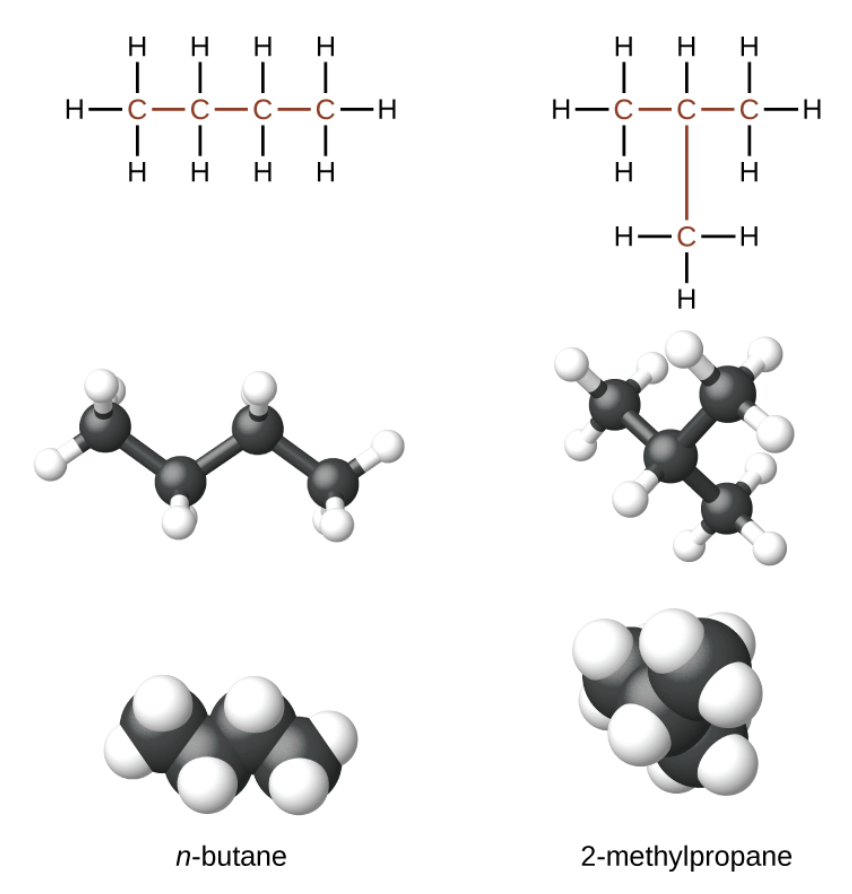
\includegraphics[width=0.5 \textwidth]{../figures/n-butane-2-methylpropane.png}
    \caption{n-butane and 2-methylpropane are structural isomers. The butane is prefixed with a
    \textit{n} as a short for the term \textit{normal} to refer to a chain of carbon atoms without
    branching}
\end{figure}

The four-carbon straight chain alkane butane may also be drawn with different bends or kinks in the
backbone because the groups can freely rotate about the C-C bonds. This doesn't change the identity
of the compound, but is rather a different representation of it

\begin{figure}[ht!]
    \centering
    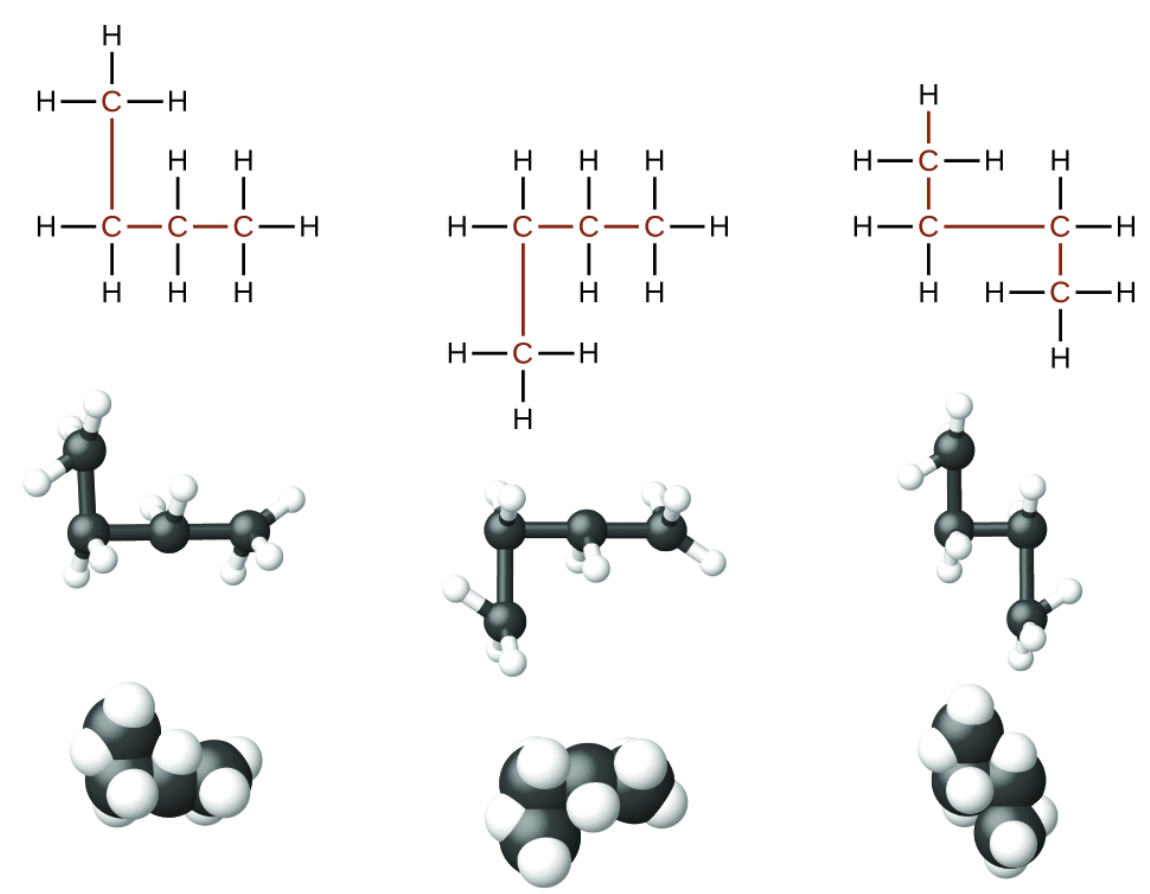
\includegraphics[width=0.6 \textwidth]{../figures/n-butane-backbones.png}
    \caption{These three representations of n-butane are not isomers because they all contain
    the same arrangement of atoms and bonds}
\end{figure}

Pentane, which has molecular formula $\ch{C5H12}$, has two branched-chain isomers, namely
isopentane and neopentane. Pentane is a straight-chain alkane, while isopentane and neopentane are
branch-chain alkanes. The prefix \textit{neo} for neopentane is from the Greek work \textit{neos},
meaning ``new''.

\begin{figure}[ht!]
    \centering
    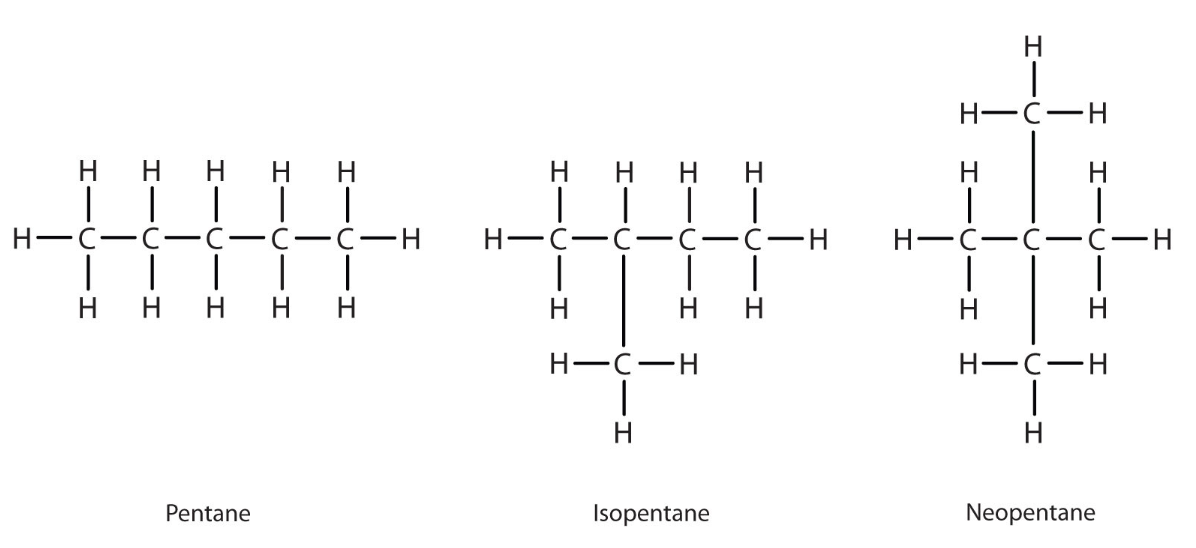
\includegraphics[width=0.8 \textwidth]{../figures/pentane-isopentane-neopentane.png}
\end{figure}

\begin{important}
    A continuous (unbranched) chain of carbon atoms is called a straight-chain even though the
    tetrahedral arrangement about each carbon is a zigzag shape. Straight-chain alkanes are sometimes
    called \textit{normal alkanes}.
\end{important}

\subsection{Naming Alkanes}
In the IUPAC system, a compound is named according to the number of carbons in the longest continuous
chain (LCC) or parent chain and the family it belongs to. Atoms or groups attached to this carbon
chain, called \textit{substituents}
\footnote{
    \textbf{Substituent:} atoms or groups of atoms that branch off the parent chain.
}
, are then named, with their positions indicated by a numerical
prefix at the beginning of the name
\[
    \text{Prefix (substituent)}-\text{Parent (\# carbons)}-\text{Suffix (family name)}
\]
\[
    \text{2-methyl}\quad\text{prop}\quad\text{ane}\to \text{2-methylpropane}
\]

\begin{table}[!ht]
    \footnotesize
    \centering
    \caption{Parent name for 1-10 carbons and example alkanes}
    \setlength{\tabcolsep}{12pt}      % column spacing
    \renewcommand{\arraystretch}{1.2} % row spacing
    \arrayrulecolor{black}            % table border color
    \begin{tabular}{l l l l}
        \rowcolor{HeaderColor}
        \# of Carbons & LCC Name & Example Alkane & Condensed Structural Formula \\ \hline
        1 & \textit{meth-} & methane & $\ch{CH4}$ \\
        2 & \textit{eth-} & ethane & $\ch{CH3CH3}$ \\
        3 & \textit{prop-} & propane & $\ch{CH3CH2CH3}$ \\
        4 & \textit{but-} & butane & $\ch{CH3CH2CH2CH3}$ \\
        5 & \textit{pent-} & pentane & $\ch{CH3CH2CH2CH2CH2CH3}$ \\ 
        6 & \textit{hex-} & hexane & $\ch{CH3CH2CH2CH2CH2CH2CH3}$ \\
        7 & \textit{hept-} & heptane & $\ch{CH3CH2CH2CH2CH2CH2CH3}$ \\
        8 & \textit{oct-} & octane & $\ch{CH3CH2CH2CH2CH2CH2CH2CH3}$ \\
        9 & \textit{non-} & nonane & $\ch{CH3CH2CH2CH2CH2CH2CH2CH2CH3}$ \\
        10 & \textit{dec-} & decane & $\ch{CH3CH2CH2CH2CH2CH2CH2CH2CH2CH3}$ \\
    \end{tabular}
\end{table}
